\documentclass[12pt, twoside]{book}
\usepackage[a4paper, margin=2.5cm, inner=4cm]{geometry}
\usepackage[usenames, dvipsnames]{color}
\usepackage{graphicx}
\usepackage{emptypage}
\usepackage{blindtext}
\usepackage{titlesec}
\usepackage{fancyhdr}
\usepackage{hyperref}
\graphicspath{ {./images} }

\renewcommand{\chaptername}{Lecture}

\titleformat
{\chapter} % command
[display] % shape
{ \normalfont\Large\bfseries} % format
{} % label
{1ex} % sep
{
    \rule{\textwidth}{1pt}
    \centering
} % before-code
[
\vspace{-1.5ex}
\rule{\textwidth}{1pt}
] % after-code

\title{\LaTeX{} Book Example}
\author{YNSRC}
\date{June 2024}

\begin{document}
\maketitle

\frontmatter %Use lowercase Roman numerals for page numbers
\chapter*{Foreword}
\addcontentsline{toc}{chapter}{Foreword}
The Foreword is written by someone who is not the book's author.

\chapter*{Preface}
\addcontentsline{toc}{chapter}{Preface}
The Preface is written by the book's author.

\tableofcontents
\listoffigures
\listoftables

\mainmatter

\chapter{Chapter One}

\section{Section One}
\blindtext[2]

\subsection{Sub-Section One}
\blindtext[3]

\subsubsection{Sub-Sub-Section One}
\blindtext[4]

\subsubsection{Sub-Sub-Section Two}
\blindtext[2]

\subsection{Sub-Section Two}
\blindtext[2]

\section{Section Two}
\blindtext[3]

\chapter{Chapter Two}

\section{Section One}
\blindtext[3]

\section{Section Two}
\blindtext

\chapter{Chapter Three}

\section{Text Formatting}
You can use \textcolor{blue}{colored} text or
\colorbox{BurntOrange}{background colored} texts. Also
\textbf{bold}, \textit{italic}, \underline{underlined} or
\texttt{typewriter font} texts or \large{large} text.

\section{Math}
$$\int_0^1{\sin x} \ dx$$

Inline symbols like $\infty$ or expressions like 
$f(x) = x^2 + 2x + 4$ also possible.

\section{Bullet List}

\begin{itemize}
    \item Item 1
    \item Item 2
    \item Item 3
    \item Item 4
    \item Item 5
\end{itemize}

\section{Numbered List}

\begin{enumerate}
    \item Item A
    \item Item B
    \item Item C
    \item Item D
\end{enumerate}

\section{Tables}

\begin{table}[h!]
    \centering
    \begin{tabular}{|c|c|} \hline
        a & b \\ \hline
        c & d \\ \hline
        e & f \\ \hline
    \end{tabular}
    \caption{Table with all borders.}
\end{table}

\vspace{12pt}

\begin{table}[h!]
    \centering
    \begin{tabular}{cc}
        a & b \\
        c & d \\
        e & f \\
    \end{tabular}
    \caption{Table with no borders.}
\end{table}

\vspace{12pt}

\begin{table}[h!]
    \centering
    \begin{tabular}{|c|c|}
        a & b \\
        c & d \\
        e & f \\
    \end{tabular}
    \caption{Table with only vertical borders.}
\end{table}

\vspace{12pt}

\begin{table}[h!]
    \centering
    \begin{tabular}{cc} \hline
        a & b \\ \hline
        c & d \\ \hline
        e & f \\ \hline
    \end{tabular}
    \caption{Table with only horizontal borders.}
\end{table}

\clearpage
\section{Figures (Images)}

\begin{figure}[h!]
    \centering
    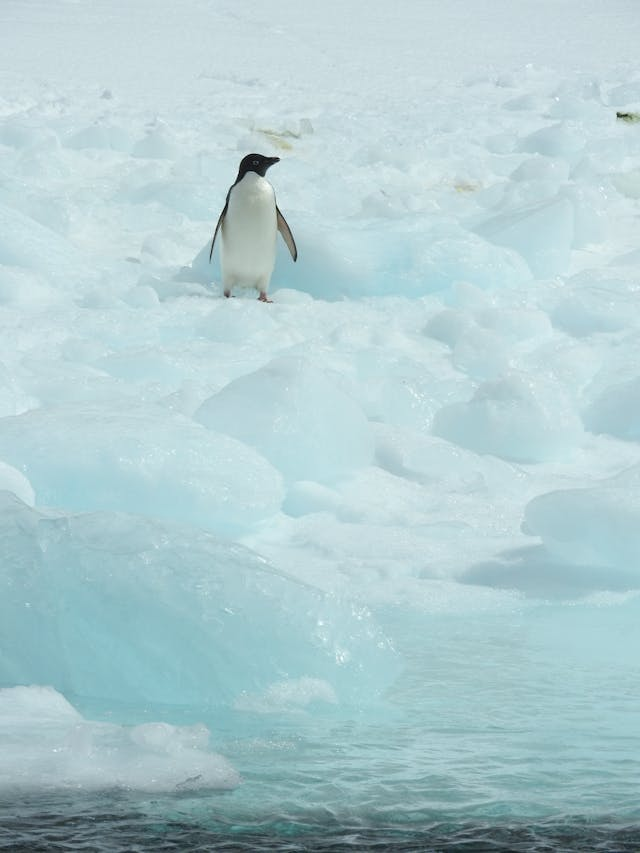
\includegraphics[scale=0.25]{penguin}
    \caption{A penguin image. Photo: 
        \href
        {https://www.pexels.com/photo/penguin-on-ice-covered-ground-4361073/}
        {David Peterson}
        .
    }
    \label{fig:enter-label}
\end{figure}

\end{document}
